

\author[Sebastian Hahn]{Nix}


\beamertemplatenavigationsymbolsempty{}

\logo{
\includegraphics[height=1cm]{Bilder/logo}}


\section{Sektion-Überschrift}

\begin{frame}
	\frametitle{Verlustfunktion (ELBO)}
	\begin{align*}
	\log\big(p_{\boldsymbol\theta}(\x)\big)
	\geq\underbrace{ \E_{\z\sim q_{\boldsymbol\phi}}\big[\log\big(\pdec\big)\big] - D_{KL}\big[\qenc||p_{\boldsymbol\theta}(\z)\big]}_{=:\ \mathrm{ELBO}\ =\ -\mathcal{L}(\boldsymbol\theta,\boldsymbol\phi,\mathbf{x}_i)}
	\end{align*}
\end{frame}

\begin{frame}
	\frametitle{Beispiel eines latenten Raumes}
	
	\begin{figure}[h!]
		\centering
		\begin{minipage}{.6\textwidth}
			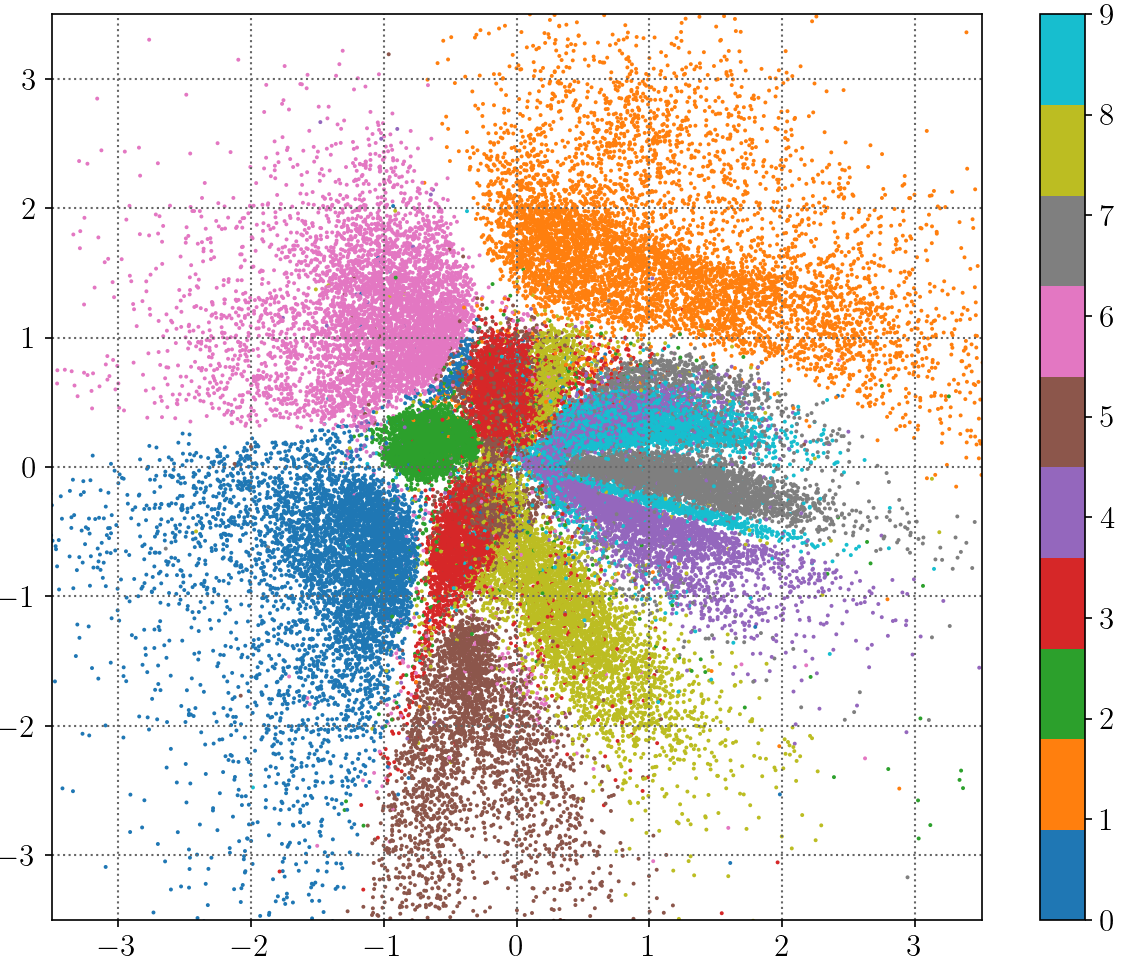
\includegraphics[scale=0.28]{Bilder/latent_space_2D.png}
		\end{minipage}%
		\begin{minipage}{.5\textwidth}
			
\includegraphics[scale=0.23]{Bilder/latent_space_2D_reconstructions.png}
		\end{minipage}
	\end{figure}
\end{frame}
